\documentclass{article}
\usepackage[utf8]{inputenc}
\usepackage{amsmath}
\usepackage{graphicx}
\usepackage{geometry}
\graphicspath{{images/} 
\geometry{legalpaper, lmargin=0.7in, bmargin=1in}}

\begin{document}
%%%%%%%%%%%%%%
%page  titre en caractères plus large
%%%%%%%%%%%%%%
\begin{titlepage}   
	\large{
		\begin{center}
			UNIVERSITÉ DE SHERBROOKE\\Faculté de génie\\
			Département de génie électrique et génie informatique\\
			\vspace{3cm}
			{\LARGE\textbf{éléments de statique et dynamique}}\\
			\vspace{2cm}
			\LARGE{Rapport APP1}\\
			\vspace{2cm}
			Présenté à\\l'équipe professorale de la session S4\\
			\vspace{2cm}
			Produit par\\Axel Bosco, Philippe Garneau, Philippe Spino\\
			\vspace{1cm}
			\vfill{7 mai 2017 - Sherbrooke}
		\end{center}
	}
\end{titlepage}
\newpage
%%%%%%%%%%%%%%
%Table des matières
%%%%%%%%%%%%%%
\tableofcontents

\newpage
\section{Introduction}
Dans le cadre de l’implémentation d’un système de commande du bras mécanique de l’entreprise CRM, il faut analyser le mouvement d’un point A sur le plan 2D de celui-ci. Le point A, situé à l’extrémité des bras du robot, bouge selon le bras BA attaché au moteur MB et le bras BA bouge selon le bras OB avec le moteur MO. Notre mandat est de déterminer les forces et les couples nécessaires pour maintenir le robot en équilibre ou de le bougé selon des directives spécifiques. Pour la résolution de la problématique, l’équipe a divisé l’ensemble en plusieurs étapes. La première étape fût de regarder la cinématique du système de manière générale, ensuite dans des cas avec des restrictions sur les mouvements possibles du point A dans le plan 2D. En deuxième partie, l’analyse est centrée sur la statique et la dynamique du système. 

\section{Cinématique}
Dans l'analyse de la cinématique, il y avait trois cas à analyser. Il faut déterminer la relation du mouvement du Point A en reliant les mouvements angulaires des bras OB et BA au mouvement linéaire du point A dans tous les cas. Précisément, il faut déterminer les vecteurs de positions, de vitesses et d’accélération linéaire du point A en fonction des longueurs des bras, soit L1 et L2, des angles $\phi$ et $\theta$ et de leur vitesse et accélération angulaires respectives.
Les calcules présenté dans la section suivant explique les démarches mathématiques utilisé pour la résolution des cas.

\subsection{équations générales}
équation générale: vecteur position

\begin{equation}
\overrightarrow{OA} = 
    l_1\Bigg[\begin{array}{cc}
    cos(\theta) \\
    sin(\theta) \\
    0
    \end{array}\Bigg]
    +
    l_2\Bigg[\begin{array}{cc}
    cos(\phi) \\
    sin(\phi) \\
    0
    \end{array}\Bigg]
\end{equation}

\noindent équation générale: vecteur vitesse

\begin{equation}
\overrightarrow{V_{OA}} = 
    l_1\Bigg[\begin{array}{cc}
    -sin(\theta)\theta' \\
    cos(\theta)\theta' \\
    0
    \end{array}\Bigg]
    +
    l_2\Bigg[\begin{array}{cc}
    -sin(\phi)\phi' \\
    cos(\phi)\phi' \\
    0
    \end{array}\Bigg]
\end{equation}

\noindent equation generale: vecteur acceleration

\begin{equation}
\overrightarrow{\alpha_{OA}} =
	l_1\Bigg[\begin{array}{cc}
	-cos(\theta)(\theta')^2-sin(\theta)\theta'' \\
	-sin(\theta)(\theta')^2+cos(\theta)\theta'' \\
	0
	\end{array}\Bigg]
	+
	l_2\Bigg[\begin{array}{cc}
	-cos(\phi)(\phi')^2-sin(\phi)\phi'' \\
	-sin(\phi)(\phi')^2+cos(\phi)\phi'' \\
	0
	\end{array}\Bigg]
\end{equation}

\subsection{Mouvement horizontal}
\subsubsection{Relation entre $\theta$ et $\phi$ lorsque $\phi$ est negatif}
Trouver $sin(\phi)$:

\begin{equation}
l_1 = l_2
\end{equation}

\begin{equation}
\overrightarrow{Y_A} = l_1sin(\theta)+l_1sin(\phi)
\end{equation}

\begin{equation}
0 = l_1sin(\theta)+l_1sin(\phi)
\end{equation}

\begin{equation}
sin(\phi) = -sin(\theta)
\end{equation}

\noindent Trouver $cos(\phi)$ a partir de $sin(\phi)$:

\begin{equation}
cos^2(\phi)+sin^2(\phi) = 1
\end{equation}

\begin{equation}
cos(\phi) = \sqrt{1-sin^2(\theta)}
\end{equation}

\subsubsection{3 equations cinematiques}
Position:

\begin{equation}
l_1 = l_2
\end{equation}

\begin{equation}
\overrightarrow{X_A} = l_1cos(\theta)+l_1\sqrt{1-sin^2(\theta)}
\end{equation}

\begin{equation}
\overrightarrow{X_A} = l_1cos(\theta)+l_1\sqrt{cos^2(\theta)}
\end{equation}

\begin{equation}
\overrightarrow{X_A} = 2l_1cos(\theta)
\end{equation}

\noindent Vitesse:

\begin{equation}
\overrightarrow{V_{Ax}} = \frac{d(2l_1cos(\theta))}{dt}
\end{equation}

\begin{equation}
\overrightarrow{V_{Ax}} = -2l_1sin(\theta)\theta'
\end{equation}

\begin{equation}
\theta' = \omega_{OB}
\end{equation}

\begin{equation}
\overrightarrow{V_{Ax}} = -2l_1sin(\theta)\omega_{OB}
\end{equation}

\noindent Acceleration:

\begin{equation}
\overrightarrow{\gamma_{Ax}} = \frac{d(-2l_1sin(\theta)\theta')}{dt}
\end{equation}

\begin{equation}
\overrightarrow{\gamma_{Ax}} = -2l_1cos(\theta)(\theta')^2-2l_1sin(\theta)\theta''
\end{equation}

\begin{equation}
\theta' = \omega_{OB}
\end{equation}

\begin{equation}
\theta'' = \alpha_{OB}
\end{equation}

\begin{equation}
\overrightarrow{\gamma_{Ax}} = -2l_1cos(\theta)(\omega_{OB})^2-2l_1sin(\theta)\alpha_{OB}
\end{equation}

\subsubsection{Courbes du mouvement horizontal}
Position:
\newline
\noindent 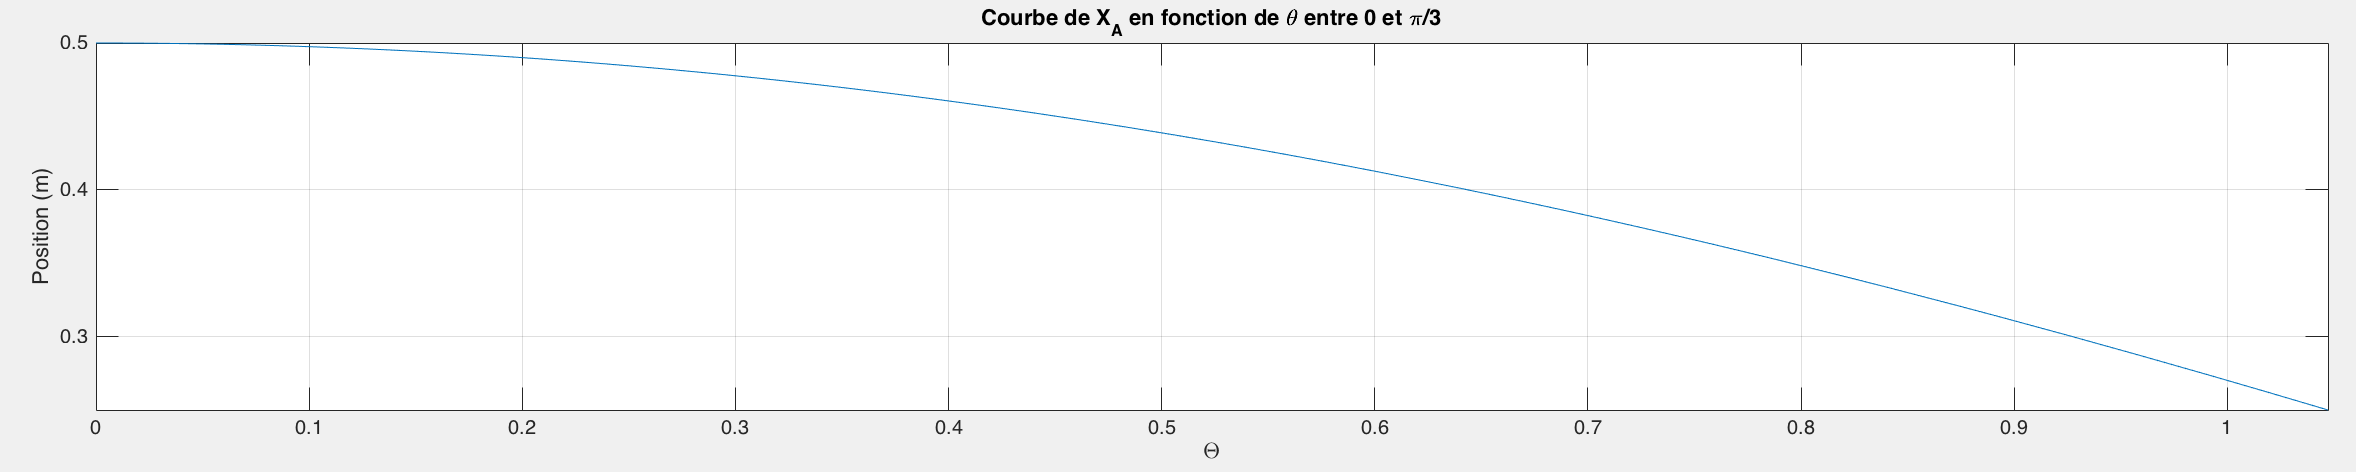
\includegraphics[width=\textwidth]{hori_pos}
BLABLA c'est une explication de ma courbe...
\newline
\newline
\noindent Vitesse:
\newline
\noindent 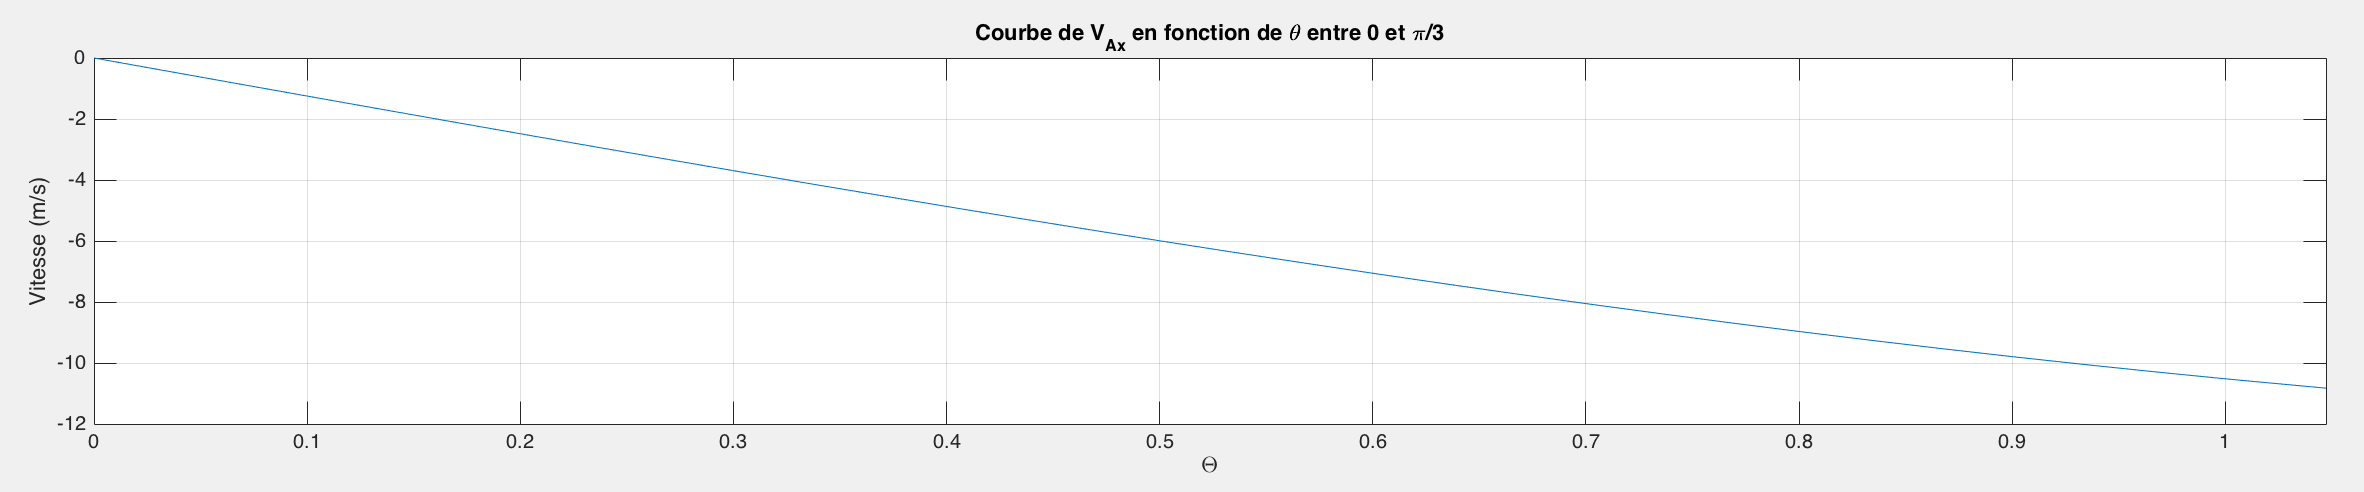
\includegraphics[width=\textwidth]{hori_vit}
BLABLA c'est une explication de ma courbe...
\newline
\newline
\noindent Acceleration:
\newline
\noindent 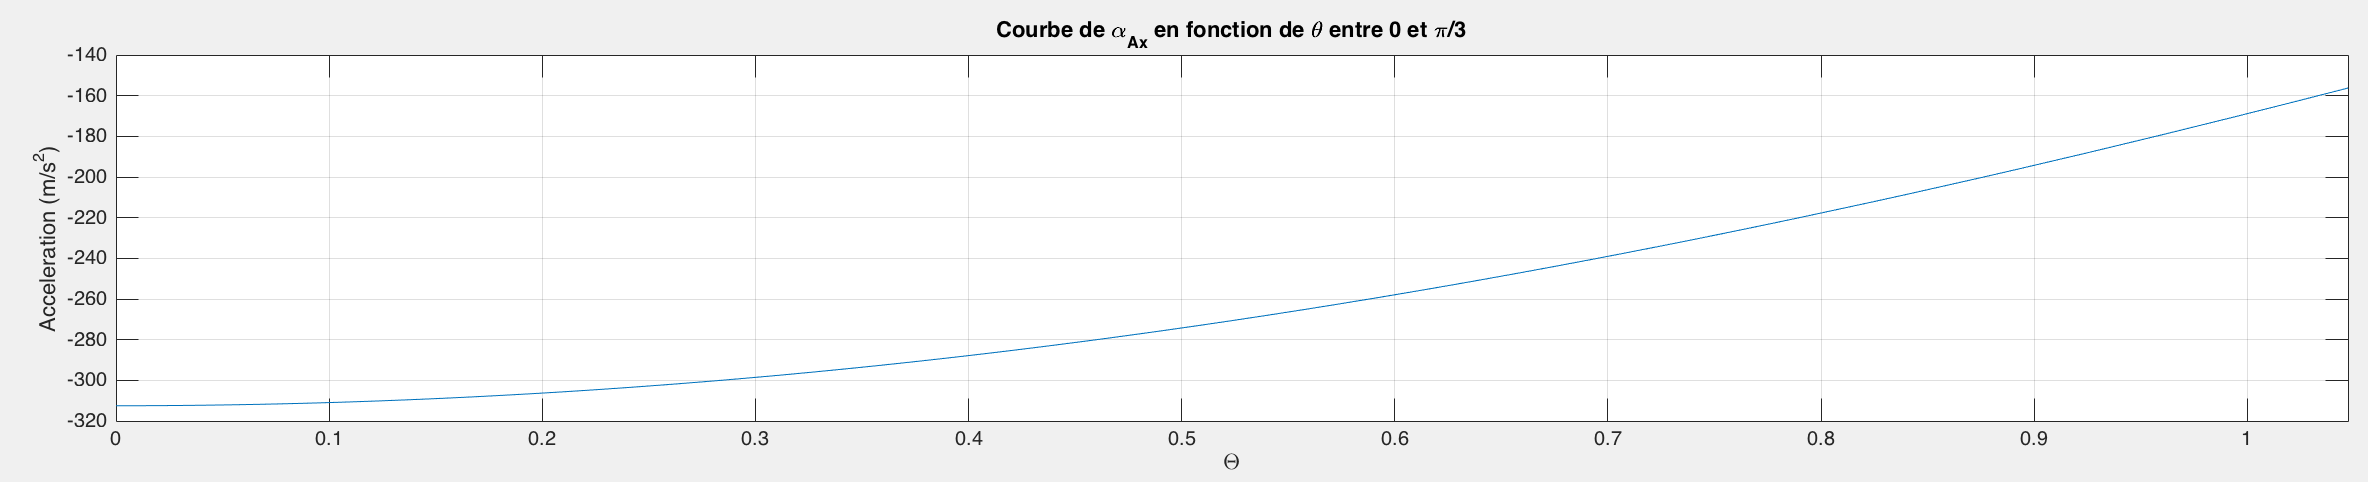
\includegraphics[width=\textwidth]{hori_accel}
BLABLA c'est une explication de ma courbe...

\subsection{Mouvement vertical}
\subsubsection{Relation entre $\theta$ et $\phi$ lorsque $\phi$ est negatif}
Trouver $cos(\phi)$:

\begin{equation}
l_1 = l_2
\end{equation}

\begin{equation}
\overrightarrow{X_A} = l_1cos(\theta)+l_1cos(\phi)
\end{equation}

\begin{equation}
l_1 = l_1cos(\theta)+l_1cos(\phi)
\end{equation}

\begin{equation}
cos(\phi) = 1-cos(\theta)
\end{equation}

\noindent Trouver $sin(\phi)$ a partir de $cos(\phi)$:

\begin{equation}
cos^2(\phi)+sin^2(\phi) = 1
\end{equation}

\begin{equation}
sin^2(\phi) = 1-cos^2(\phi)
\end{equation}

\begin{equation}
sin^2(\phi) = -cos^2(\theta)+2cos(\theta)
\end{equation}

\begin{equation}
\pm sin(\phi) = \sqrt{-cos^2(\theta)+2cos(\theta)}
\end{equation}

\noindent Nous considerons que $\phi$ est negatif, donc:

\begin{equation}
sin(\phi) = -\sqrt{-cos^2(\theta)+2cos(\theta)}
\end{equation}

\subsubsection{2 equations cinematiques}
Position:

\begin{equation}
l_1 = l_2
\end{equation}

\begin{equation}
\overrightarrow{Y_A} = l_1sin(\theta)-l_1\sqrt{-cos^2(\theta)+2cos(\theta)}
\end{equation}

\noindent Vitesse:

\begin{equation}
\overrightarrow{V_{Ay}} = \frac{d(l_1sin(\theta)-l_1\sqrt{-cos^2(\theta)+2cos(\theta)})}{dt}
\end{equation}

\begin{equation}
\overrightarrow{V_{Ay}} = l_1cos(\theta)\theta'-\\
\frac{l_1(-cos^2(\theta)+2cos(\theta))'}{2\sqrt{-cos^2(\theta)+2cos(\theta)}}
\end{equation}

\begin{equation}
\overrightarrow{V_{Ay}} = l_1cos(\theta)\theta'-\\
\frac{l_1sin(\theta)(cos(\theta)-1)\theta'}{\sqrt{-cos^2(\theta)+2cos(\theta)}}
\end{equation}

\begin{equation}
\theta' = \omega_{OB}
\end{equation}

\begin{equation}
\overrightarrow{V_{Ay}} = l_1cos(\theta)\omega_{OB}-\\
\frac{l_1sin(\theta)(cos(\theta)-1)\omega_{OB}}{\sqrt{-cos^2(\theta)+2cos(\theta)}}
\end{equation}

\subsubsection{Courbes du mouvement vertical}
Position:
\newline
\noindent 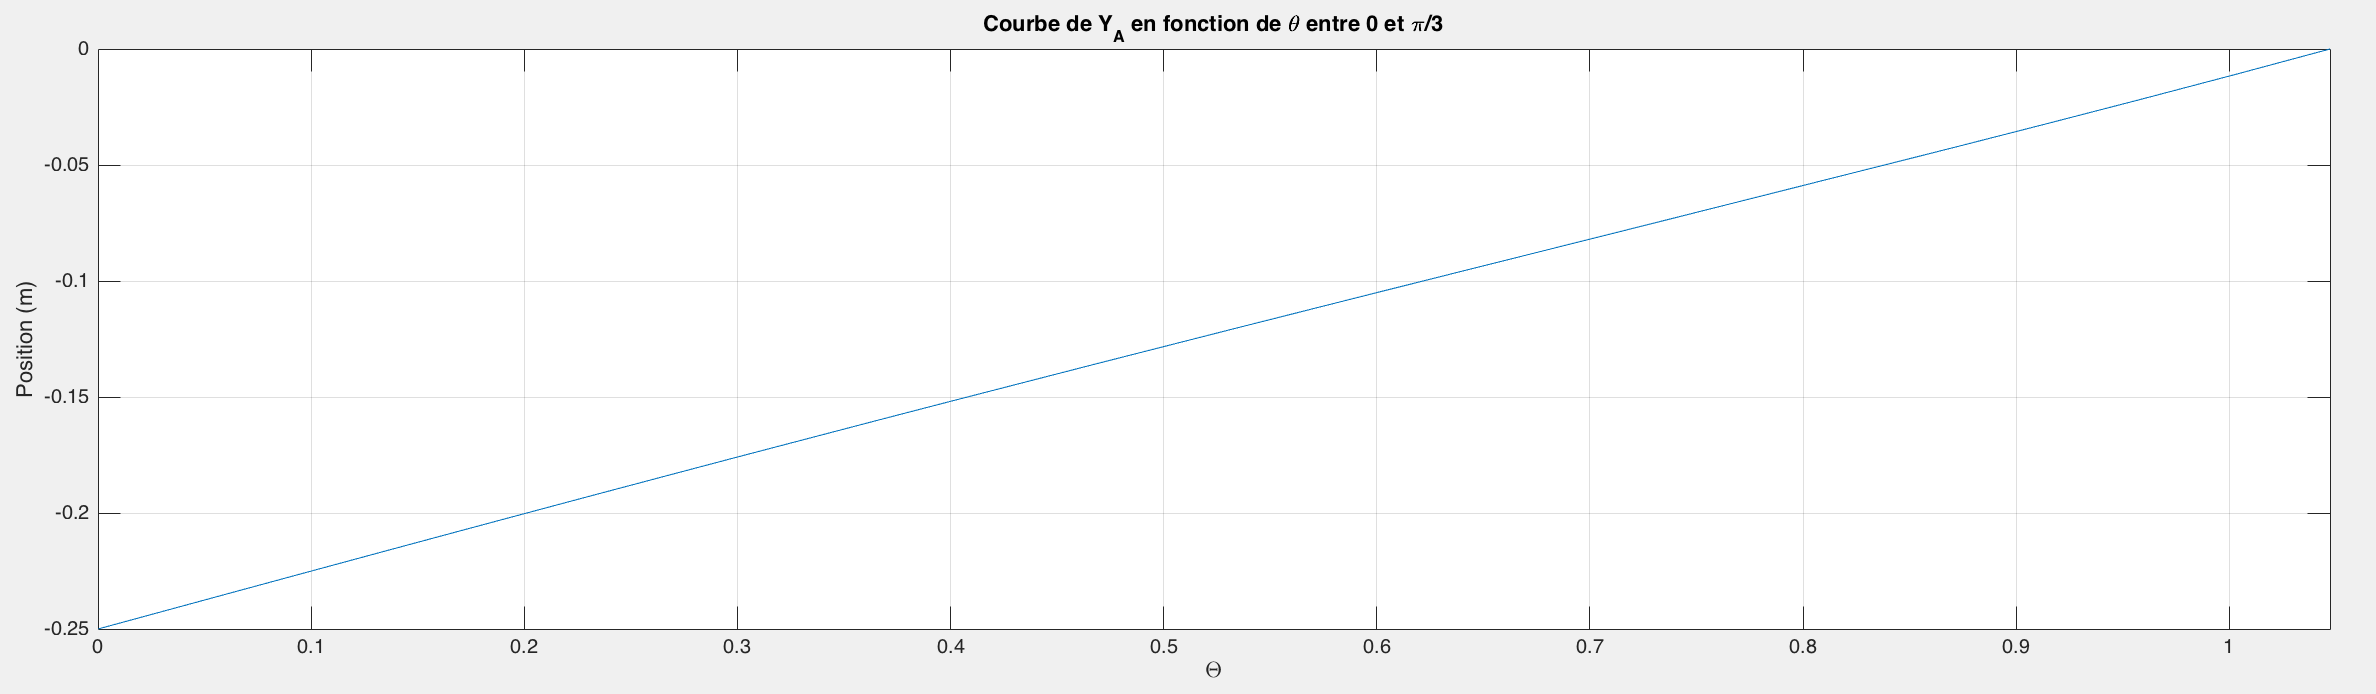
\includegraphics[width=\textwidth]{vert_pos}
BLABLA c'est une explication de ma courbe...
\newline
\newline
\noindent Vitesse:
\newline
\noindent 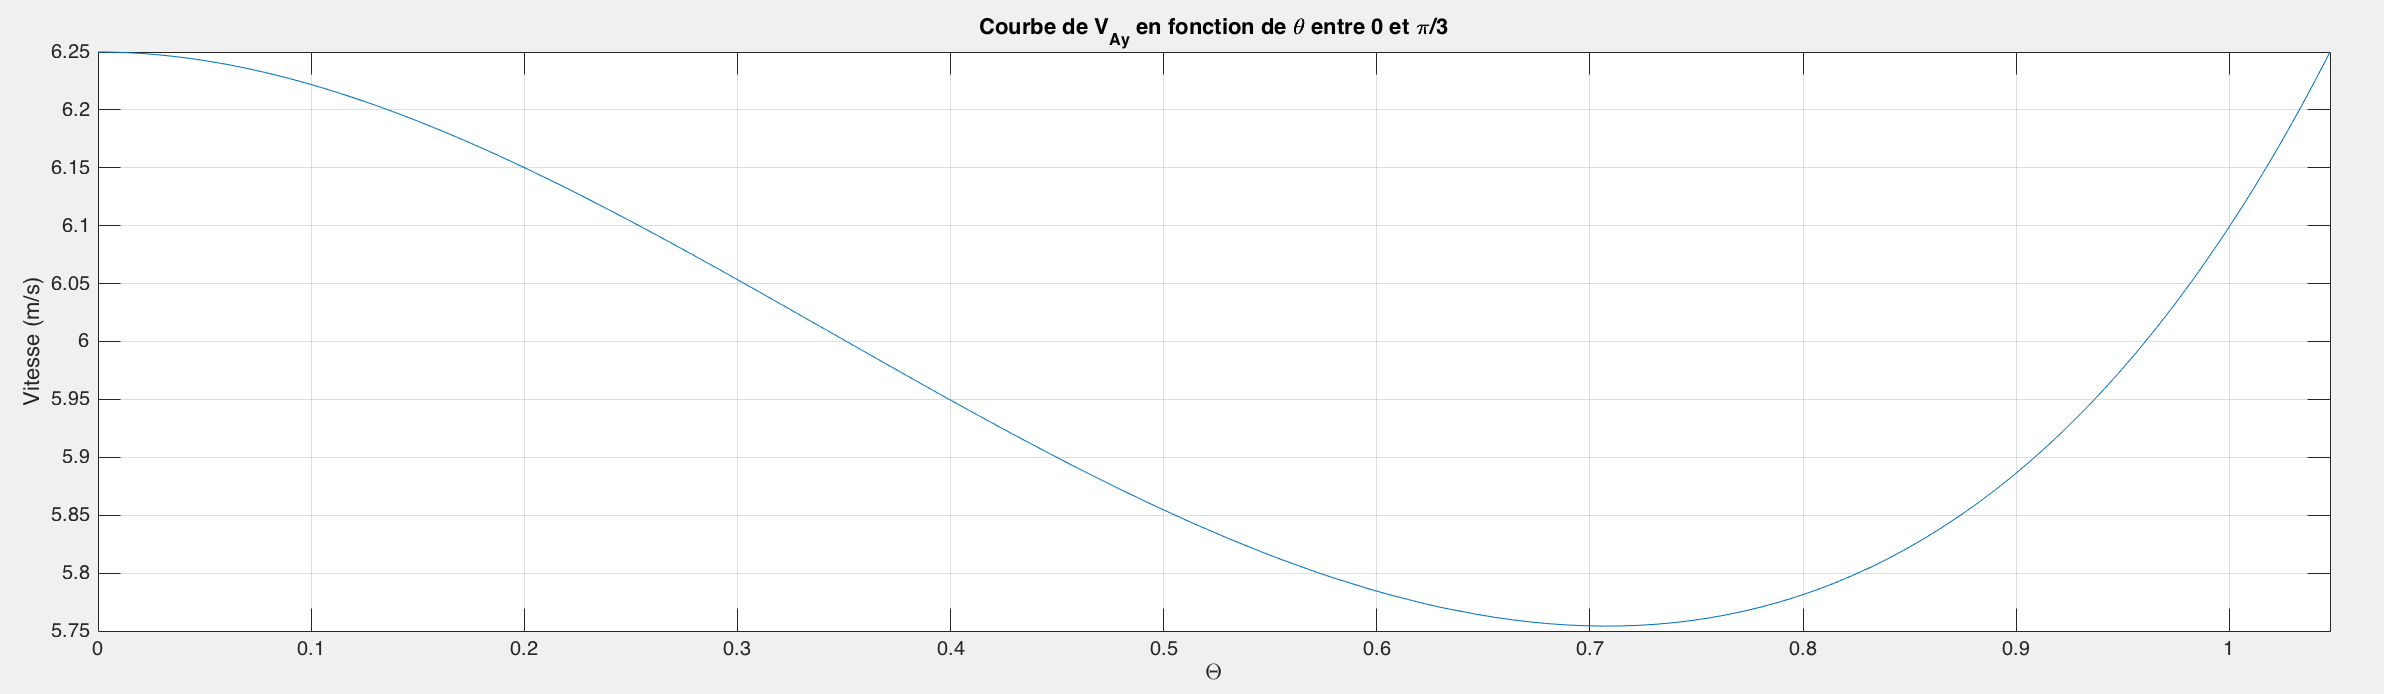
\includegraphics[width=\textwidth]{vert_vit}
BLABLA c'est une explication de ma courbe...

\subsection{Relation entre $\theta$ et $\phi$ et les commandes de $M_O$ et $M_B$}
Lorsque le moteur $M_B$ s'active, il affecte seulement la valeur de $\phi$. Par contre, lorsque le moteur $M_O$ s'active, il vient bien evidemment modifier la valeur de $\theta$, mais aussi la valeur de $\phi$, car les tiges OB et BA peuvent etre consideree comme une seule tige OA lorsque seulement le moteur $M_O$ est en marche.

\section{Statique et Dynamique}
Pour l'analyse du système dans le domaine du statique, on considère le cas ou le robot porte un objet $O_A$ au point A. Pour simplifier l'analyse, les tiges, représenté par les vecteurs $\overrightarrow{OB}$ et $\overrightarrow{BA}$, sont approximés par des tiges minces et uniformes, les moteurs $M_O$, $M_B$ et $O_A$ sont approximés par des sphères de dimensions négligeables par rapport a OB et BA. On considère aussi que la force FB et le couple CB sont exercés sur l’extrémité B de la tige BA. FB est appliquée par OB alors que CB est appliqué par MB.

\subsection{Statique}
Dans le domaine statique, on fait l'étude du système a l'équilibre. C'est a dire lorsque: 
\begin{equation}
\sum \overrightarrow{F_{ext}} = 0
\end{equation}

\begin{center} 
et quand:
\end{center}

\begin{equation}
\sum \overrightarrow{M_B} = 0
\end{equation}
\newline
\noindent 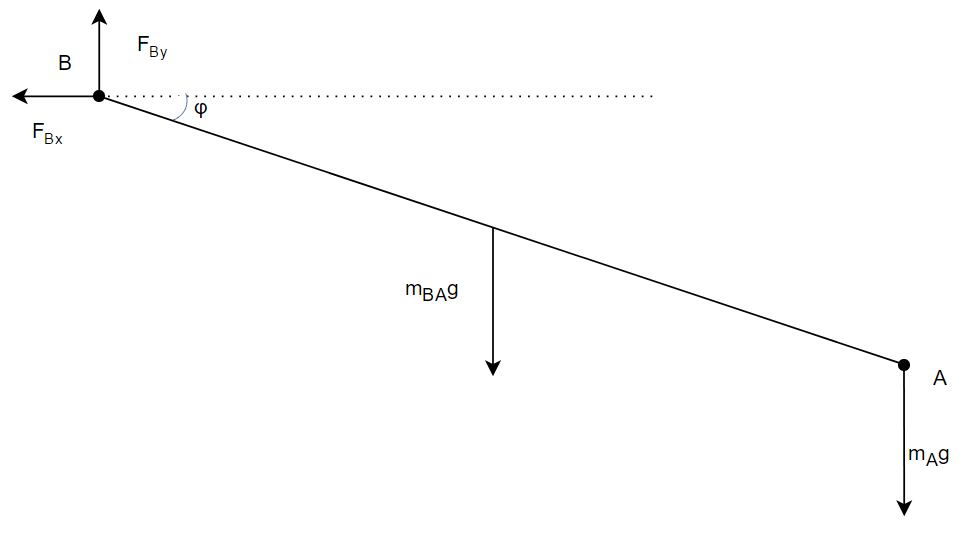
\includegraphics[width=\textwidth, scale = 0.01]{DCL_BA}
\begin{center}
DCL du bras BA:
\end{center}

En appliquant les forces dans le Diagramme des Corps Libres, l'équation suivant est obtenu:

\begin{equation}
\sum \overrightarrow{F_{ext}} = -m_{BA}.\overrightarrow{g} -m_A.\overrightarrow{g} + \overrightarrow{F_B}
\end{equation}

\begin{equation}
\sum F_x = -m_{BA}.g_x -m_A.g_x + F_{B_x} = 0
\end{equation}

\begin{equation}
\sum F_y = -m_{BA}.g_y -m_A.g_y + F_{B_y} = 0
\end{equation}

Dans l'équation 41, il n'est pas nécessaire de calculer la valeur de $F_{B_x}$ car celle-ci vaut 0. Cela veut dire qu'il ne reste que $F_{B_y}$ comme force.

\begin{equation}
\ F_{B_y} = m_A.g + m_{BA}.g
\end{equation}

Il reste maintenant qu'a trouver la somme des moments de forces $\sum \overrightarrow{M_B}$.

\begin{equation}
\sum \overrightarrow{M_B} = -lm_Acos(\phi) - \frac{l}{2}m_{BA}gcos(\phi) + C_B = 0
\end{equation}

ce qui nous donne le couple $C_B$ suivant: 

\begin{equation}
\ C_B = lm_Acos(\phi)+ \frac{l}{2}m_{BA}gcos(\phi)
\end{equation}

\subsection{Dynamique}
Dans l'analyse du domaine dynamique du système, il faut faire l'étude du mouvement engendré par le moteur $M_O$. En regardant le Diagramme Cinétique du bras BA, on peut déterminer $F_B$ et $C_B$ en fonction de l'angle $\phi$, de $l$ dans le cas ou BA tourne avec une accélération angulaire constante $\alpha_{BA}$ pendant que OB est immobile.

\begin{equation}
\sum \overrightarrow{F_{ext}} = m_{BA}.\gamma_{G_{BA}} + m_A.\gamma_{G_A} + \overrightarrow{F_B}
\end{equation}

\begin{equation}
    \Bigg[\begin{array}{cc}
    F_{B_x} \\
    F_{B_y} \\
    0
    \end{array}\Bigg]
    =
    m_{BA}\Bigg[\begin{array}{cc}
    -\omega^2_{BA}\frac{l}{2} \\
    \alpha_{BA}\frac{l}{2} \\
    0
    \end{array}\Bigg]
    +
    m_A\Bigg[\begin{array}{cc}
    -\omega^2_{BA}l \\
    \alpha_{BA}l \\
    0
    \end{array}\Bigg]
\end{equation}

Ensuite, un projection est fait:

\begin{equation}
\ F_{B_x} = \frac{-m_{BA}\omega_{BA}l}{2} - m_A\omega_{BA}l 
\end{equation}

\begin{equation}
\ F_{B_y} = m_{BA}\alpha_{BA} + m_A\alpha_{BA}l + m_{BA}g + m_Ag
\end{equation}

\noindent En ce qui concerne la somme des moments d'inertie, 

\begin{equation}
\sum \overrightarrow{M_A} = I_A\alpha_A + I_{BA}\alpha_{BA}
\end{equation}

\begin{equation}
\ I_A\alpha_A + I_{BA}\alpha_{BA} = C_B - M_B - M_A
\end{equation}

\begin{equation}
\ C_B = alpha_A + I_{BA}\alpha_{BA} + M_B + M_A
\end{equation}

\begin{equation}
\ C_B = (ml^2 + \frac{ml^2}{3})\alpha{BA}+ m_{BA}g\frac{l}{2}cos(\phi) + m_Aglcos(\phi)
\end{equation}

\subsection{Courbes Obtenue de Statique et de Dynamique}
Statique:
\newline
\noindent 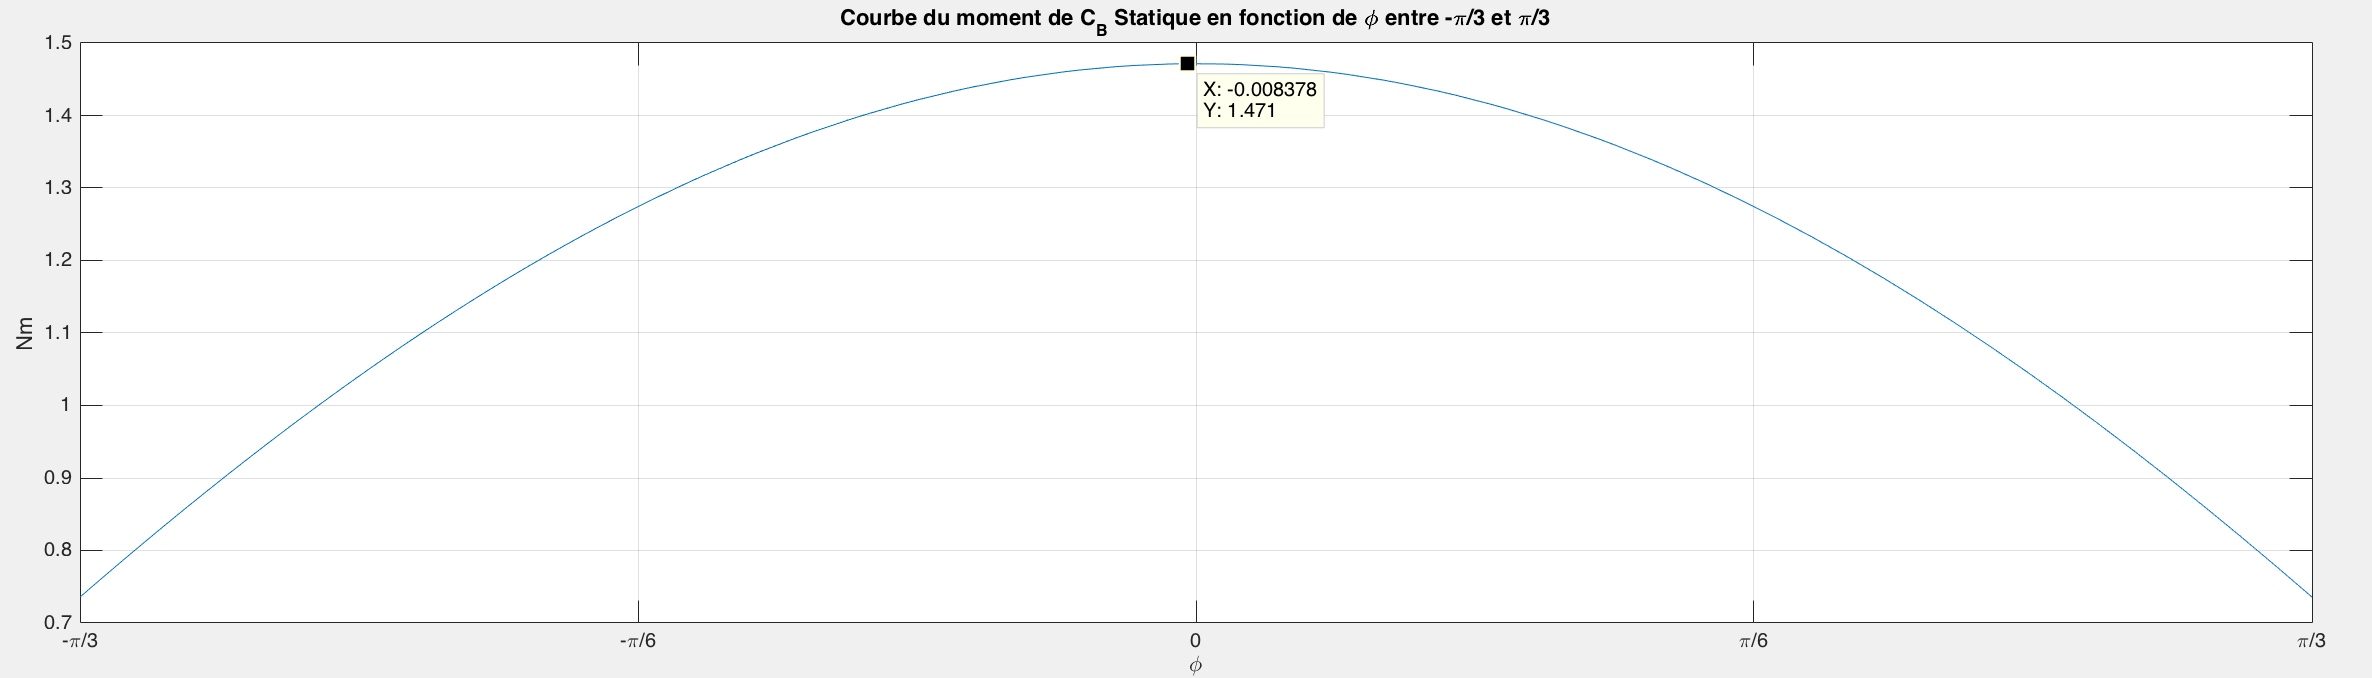
\includegraphics[width=\textwidth]{statique}
\newline
\noindent Dynamique:
\newline
\noindent 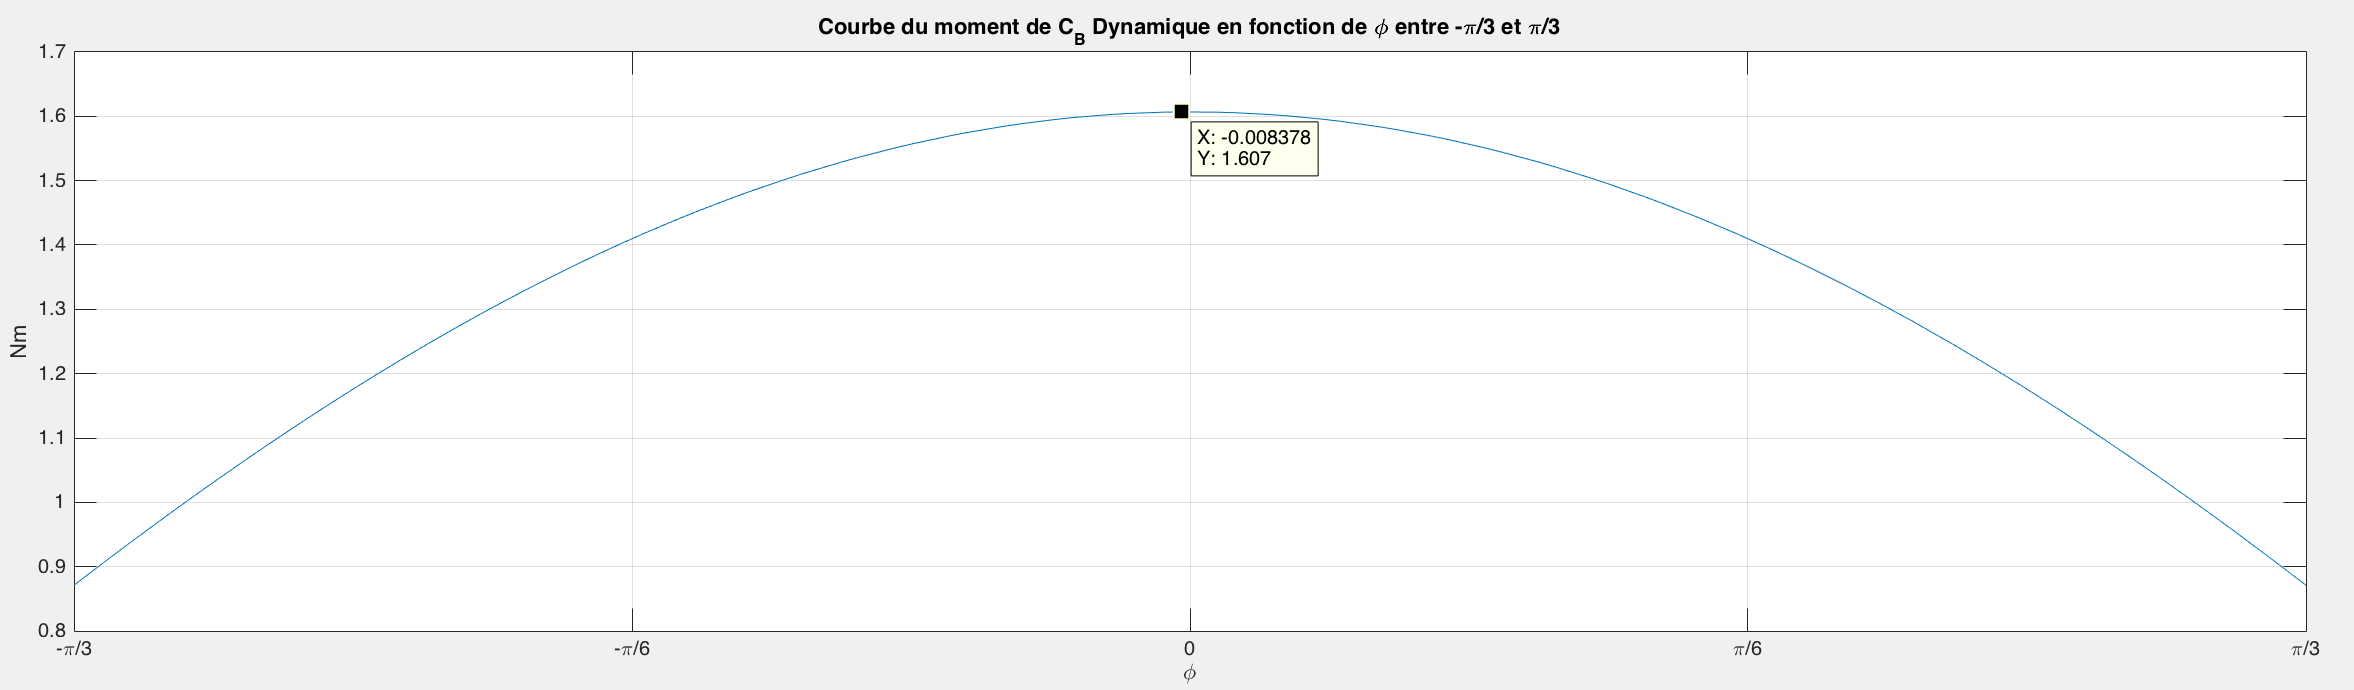
\includegraphics[width=\textwidth]{dynamique}

\subsubsection{Analyse des courbes de Statique et Dynamique}
Très rapidement, il peut être observé que les deux courbes ont une forme extrêmement similaire. On dirait que les valeurs retrouvées dans la courbe en statique ont été translatées vers le haut sur l'ordonnée. Ceci peut être expliqué par le simple fait qu'en dynamique, il faut une force pour contrer les effets de la gravite (statique) ainsi qu'une force additionelle pour simplement bouger notre bras (dynamique). La force requise pour bouger le bras reste pareille à tout moment et ne fait que s'additioner à la force variable requise pour tenir le bras en équilibre. C'est pour ça que la courbe représentant la dynamique semble avoir seulement reçu une translation positive sur l'ordonnée.

Donc, pour bien représenter le système du bras BA, le schéma suivant démontre l'ensembles des forces appliqués dans le système.


\end{document}